\documentclass[xcolor=svgnames]{beamer}

\usepackage{bera}
\usepackage[utf8]    {inputenc}
\usepackage[T1]      {fontenc}
\usepackage[english] {babel}

\usepackage{amsmath,amsfonts,graphicx}
\usepackage{beamerleanprogress}

\title
	[Escalabilidad de SDN en la RAU]
  {Proyecto de grado \\
  	Escalabilidad de Redes Definidas por Software en la Red Académica}

\author
	[Santiago Vidal]
  {Santiago Vidal \\
  	{\normalfont Tutores: \\
  	Dr. Eduardo Grampín \\
  	MSc. Martín Giachino}}

\date
  {5 de octubre de 2016}

\institute
  [UdelaR]
  {Instituto de Computación \\
  	Facultad de Ingeniería \\
  	Universidad de la República}


\begin{document}

% Directorio con las imagenes
\graphicspath{{Figs/}}

\maketitle

\section{Agenda}

\begin{frame}{Agenda}

  \begin{itemize}
	  \item Introducción
	  \item Conceptos previos \& RAUFlow
	  \item Entorno virtual
	  \item Pruebas de escala
	  \item Conclusiones
  \end{itemize}
\end{frame}

\section{Introducción}

\begin{frame}{}
	\begin{center}
		\huge{Introducción}
	\end{center}
\end{frame}

\begin{frame}{Diapo1}
	
\end{frame}

\begin{frame}{Diapo2}
	
\end{frame}

\begin{frame}{Diapo3}
	
\end{frame}

\begin{frame}{Diapo4}
	
\end{frame}





\section{Conceptos previos \& RAUFlow}

\begin{frame}{}
	\begin{center}
		\huge{Conceptos previos}
	\end{center}
	\begin{center}
		\huge{\&}
	\end{center}
	\begin{center}
		\huge{RAUFlow}
	\end{center}
\end{frame}

\begin{frame}{Diapo1}
	
\end{frame}





\section{Entorno virtual}

\begin{frame}{}
	\begin{center}
		\huge{Entorno virtual}
	\end{center}
\end{frame}

\begin{frame}{Objetivo}
	Poder utilizar la arquitectura RAUFlow y RAUSwitch en un entorno virtual, para poder hacer experimentos y pruebas.
\end{frame}
%Pruebas y experimentos que no son posibles con prototipos físicos. Incluso si se contara con todo el equipamiento, la configuración es muy compleja.

\begin{frame}{Requerimientos}
	Requerimientos funcionales:
	\begin{enumerate}
		\item RAUSwitch virtuales:
		\begin{enumerate}
			\item OpenFlow 1.3
			\item OSPF
			\item SNMP (no esencial)
		\end{enumerate}
		\item Hosts virtuales
		\item Controlador RAUFlow
	\end{enumerate}
	\pause
	Requerimientos no funcionales:
	\begin{enumerate}
		\item Configurabilidad / Usabilidad
		\item Escalabilidad
	\end{enumerate}
\end{frame}

\begin{frame}{Siguiente paso}
	\begin{center}
		Se descarta una construcción desde cero
	\begin{figure}[t]
		
\includegraphics[scale=0.1]{arrow_down}
	\end{figure}
	Hay que encontrar una herramienta que cumpla los requerimientos
	\end{center}
\end{frame}

\begin{frame}{Elección de una herramienta}
	\begin{alertblock}{Herramientas orientadas a SDN}
		\begin{itemize}
			\item Algunas no soportan OpenFlow 1.3
			\item Algunas no permiten un controlador externo.
			\item \textbf{Ninguna contempla switches híbridos!}
		\end{itemize}
	\end{alertblock}
	\pause
	\begin{block}{Herramientas de propósito general}
		\begin{itemize}
			\item Algunas no tienen buena configurabilidad.
			\item La \textbf{escalabilidad} es un gran problema.
		\end{itemize}
	\end{block}
\end{frame}

\begin{frame}{Mininet}
	\begin{itemize}
		\item Emulador de redes.
		\item Comúnmente utilizado para experimentar con SDN y OpenFlow.
		\item Virtualización ligera (containers).
		\item Cumple todos los requerimientos \textbf{excepto} el concepto de los switches híbridos.
	\end{itemize}
	\pause
	{\color{green}Solución: utilizar Mininet pero como emulador de propósito general.}
\end{frame}

\begin{frame}{Arquitectura de Mininet}
	\begin{figure}[t]
		\centering
		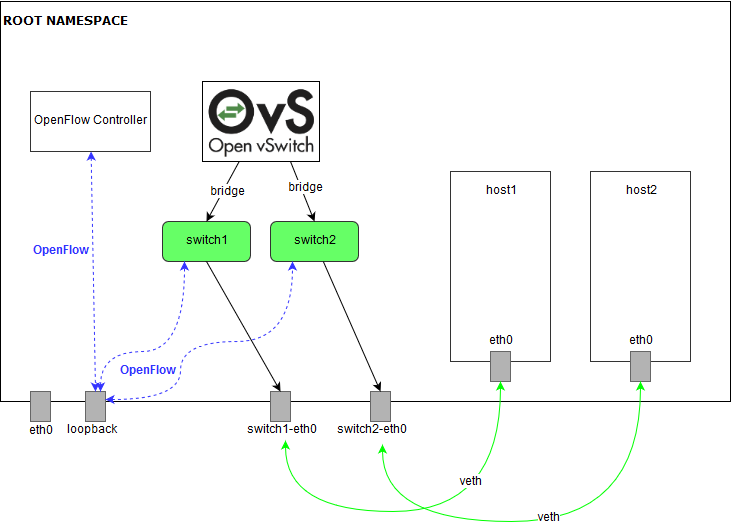
\includegraphics[scale=0.5]{mininet_architecture}
	\end{figure}
\end{frame}
% Los recursos de red de cada switch no están aislados entre sí.

\begin{frame}{Diseño e implementación}
	
\end{frame}

\begin{frame}{Ventajas}
	\begin{itemize}
		\item Utiliza las mismas herramientas que el prototipo físico. Podría utilizarse incluso en conjunto con dispositivos físicos.
	\end{itemize}
\end{frame}



\section{Pruebas de escala}

\begin{frame}{}
	\begin{center}
		\huge{Pruebas de escala}
	\end{center}
\end{frame}

\begin{frame}{Diapo1}
	
\end{frame}





\section{Conclusiones}

\begin{frame}{}
	\begin{center}
		\huge{Conclusiones}
	\end{center}
\end{frame}

\begin{frame}{Diapo1}
	
\end{frame}

%\begin{frame}
%  {A Movie}
%
%  \begin{block}{Some block}
%    \begin{itemize}
%    \item Movies only seem to work in Adobe Reader
%    \item Movie file is not embedded, it must be on the computer
%    \end{itemize}
%  \end{block}
%
%  \begin{exampleblock}{Some more block}
%    Movies only seem to work in Adobe Reader\par
%    Movie file is not embedded, it must be on the computer
%  \end{exampleblock}
%
%  \begin{alertblock}{}
%    Some text in here.
%    \begin{itemize}
%    \item Movies only seem to work in Adobe Reader
%    \item Movie file is not embedded, it must be on the computer
%    \end{itemize}
%  \end{alertblock}
%\end{frame}


%\begin{frame}
%  {Credits}
%
%  \begin{itemize}
%  \item Brought to you by Cédric Mauclair
%  \item Please let me know about improvements!
%  \item inspiration: \url{http://www.shawnlankton.com}... (in code)
%  \end{itemize}
%\end{frame}
%
%
%\begin{frame}
%  {Questions}
%
%  \nocite{lorem,ipsum}
%  \bibliographystyle{plain}
%  \bibliography{demo}
%
%\end{frame}

\end{document}

